\subsection{Varational Principle}
If we have 1 dimensional motion of a particle with mass $m$ in a potential $V(x)$, then we can define a Lagrangian:
\begin{align*}
	\mathcal{L}(x,\dot{x}) &= \frac{m}{2}\dot{x}^2  - V(x)
\end{align*}
From which we can say:
\begin{align*}
	\frac{d}{dt} \partder{\mathcal{L}}{\dot{x}} &= \partder{\mathcal{L}}{x} \\
	m\ddot{x} &= -\frac{dV}{dx}
\end{align*}
We can also talk about our action $S = \int dt \mathcal{L}(\dot{x},x)$ which is a functional acting on our paths.
In Newtonian mechanics we can define our varaitional principle as: of all curves connecting $x_a,t_a$ to $x_b,t_b$, then the paths that extrimize the action satisfy Lagrange's equation.

The extrema of $f(x,x^2,\ldots,x^n)$ is where all partial derivitives $\partial_x^a f$ vanish, in other words:
\begin{align*}
	\delta f  &= \sum_a \partial_x^a f \delta x^a = 0
\end{align*}
We would now like to compute the variation of our action:
\begin{align*}
	\delta S[x(t)] &= \int dt \left[\partder{\mathcal{L}}{\dot{x}} \delta \dot{x} + \partder{\mathcal{L}}{x}\delta x\right] \\
	\delta S[x(t)] &= \int dt \left[- \frac{d}{dt}\partder{\mathcal{L}}{\dot{x}} + \partder{\mathcal{L}}{x}\right]\delta x
\end{align*}

\section{Special Relativity}
The speed of light is initially derived from Maxwell's equations. Initially it was theorized that there was an ``ether'' in which the speed of light was a constant, because under Galilean relativity velocities would change without an ether.
The Michaelson-Morely experiment disproved the notion of an ether, and lead to the formation of special relativity.

\subsection{Simultaneous events}
In Galilean relativity/Newtonian mechanics it is clear that you can label whether or not events are simultaneous.

We now move to labeling events in spacetime $(t,x,y,z)$.

For any worldline we can restrict the slope to be less than or equal to 1 because:
\begin{align*}
	\frac{d (ct)}{dx} &= \frac{c}{v_x} \leq 1
\end{align*}

\begin{figure*}[h]
	\centering
	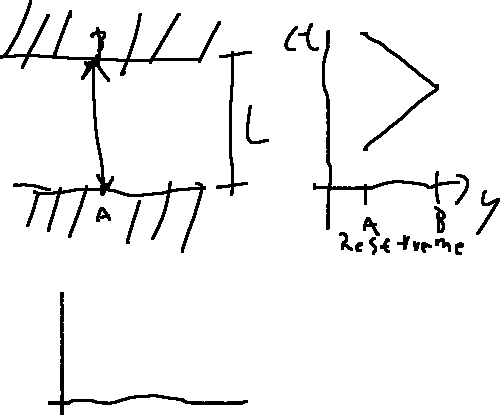
\includegraphics[width=10cm]{1-09-1.png}
	\caption*{Diagram of worldlines for the mirrors}
\end{figure*}
In an inertial frame if we consider two mirrors, then we see the round trip time will be $\Delta t = \frac{2L}{c}$. We can alos condsider this in a boosted frame, moving at a velocity $v$ in parallel to the surface of the mirrors, we see:
\begin{align*}
	\Delta x' &= v \Delta t' \\
	D &= 2\sqrt{L^2 + \left(\frac{\Delta x'}{2}\right)^2} \\
	\Delta t' &= \frac{2}{c}\sqrt{L^2 + \left(\frac{\Delta x'}{2}\right)^2}
\end{align*}

If we now consider the quantity $-(c\Delta t)^2 + (\delta \bm{r})^2$ in each coordinate system. In the boosted frame:
\begin{align*}
	-(c\Delta t')^2 + (\Delta x')^2 &= -4 (L^2 + \frac{\Delta x'\ ^2}{4}) + \Delta x'\ ^2 \\
	-(c\Delta t')^2 + (\Delta x')^2 &= -4 L^2 \\
	-(c\Delta t')^2 + (\Delta x')^2 &= -(c\Delta t)^2
\end{align*}
So it is the same in both frames.

This introduces the principle of relativity which say that our line element that defines distince have the same form in all inertial frames. In flat spacetime this line element is the one chosen above:
\begin{align*}
	ds^2 = -(c dt)^2 + dx^2 + dy^2 + dz^2
\end{align*}
Which we refer to as Minkowski space/the Minkowski line element.

From now on lowercase letters refer to spacetime, and uppercase letters refer to just space.

We say that particles with mass move along time-like world lines.

To measure distance along the worldline we'll use a ``proper time'' $\tau$ where $d\tau^2 = -\frac{ds^2}{c^2}$. We can say that two events are spacelike seperated if $(\Delta s)^2 >0$, timelike seperated if $(\Delta s)^2 <0$, and null for $(\Delta s)^2 =0$.

\subsection{Lorentz Boosts}
We will soon start dropping the factors of $c$ in many equations accepting the convention that $c=1$. 
In order to handle changing frames with a constant velocity between them, we need to use what's known as the Lorentz boost to transform instead of our simple Galilean boost.
This transformation will mix spatial and temporal dimensions in a manner somewhat analagous to rotations in Euclidean geometry:
\begin{align*}
	ct' &= \cosh\theta ct - \sinh\theta x \\
	x' &= -\sinh\theta ct + \cosh\theta x \\
	y' &= y \\
	z' &=z
\end{align*}
If we look at a worldline of a stationary particle in the boosted frame, we can see it corresponds to a constant velocity of $c\tanh\theta$ in the unboosted frame. Since $\cosh^2\theta -\sinh^2\theta = 1$ we can see:
\begin{align*}
	t' &= \gamma\left(t - \frac{vx}{c^2}\right) \\
	x' &= \gamma\left(x - v t\right) \\
	y' &= y \\
	z' &= z
\end{align*}
If we take the small velocity limit $v \ll c$, then:
\begin{align*}
	t' &= t \\
	x' &= x - v t \\
	y' &= y \\
	z' &= z
\end{align*}

We will now additionally add the conventions that we will use throughout the class. 
We will use the zeroeth index to refer to time throughtout the class, and will additionally use the einstein summation notation, i.e. $a^\alpha \hat{e}_\alpha = \sum_\alpha a^\alpha \hat{e}_\alpha$. 
We will also use greek indicies for all 4 spacetime coordinates, and latin indicies for only the spatial components.

The Lorentz boost of a vecotr is:
\begin{align*}
	a^t\ ' &= \gamma(a^t - va^x) \\
	a^x\ ' &= \gamma(a^x - va^t) \\
	a^y\ ' &= a^y \\
	a^z\ ' &= a^z
\end{align*}
And a scalar product is defined:
\begin{align*}
	\bm{a}\cdot\bm{b} &= (a^\alpha b^\beta) (\hat{e}_\alpha\cdot \hat{e}_\beta) \\
	\bm{a}\cdot\bm{b} &= (a^\alpha b^\beta) \eta_{\alpha\beta}
\end{align*}
Where for minkowski space:
\begin{align*}
	\eta_{\alpha\beta} &= \begin{pmatrix}
		-1 & 0 & 0 & 0 \\
		0 & 1 & 0 & 0 \\
		0 & 0 & 1 & 0 \\
		0 & 0 & 0 & 1
			      \end{pmatrix}
\end{align*}
So in flat space:
\begin{align*}
	\bm{a}\cdot\bm{b} &= -a^tb^t + a^x b^x + a^y b^y + a^z b^z
\end{align*}

When talking about worldilines we will typically refer to the position as a function of proper time, and a four velocity $u^\alpha = \frac{d x^\alpha}{d\tau}$. This can be written in terms of the three velocity:
\begin{align*}
	u^t &= \frac{dt}{d\tau} \\
	u^t &= \frac{1}{\sqrt{1-v^2}} \\
	u^i &= \frac{dx^i}{d\tau} \\
	u^i &= \frac{v^i}{\sqrt{1-v^2}} \\
	u^\alpha &= (\gamma,\gamma v^i)
\end{align*}

If we now compute the magnitude of $u^\alpha$, i.e. $u_\alpha u^\alpha = -1$

\subsection{Dynamics}
In the abscencce of outside forces, we should have constant 4 velocities, so (in any inertial frame):
\begin{align*}
	\frac{d u^\alpha}{d\tau} &= 0
\end{align*}
If we have a force applied though we see:
\begin{align*}
	m\frac{d u^\alpha}{d\tau} &= f^\alpha
\end{align*}
We say this is a 4 acceleration $a^\alpha = \frac{d u^\alpha}{d\tau}$, so we have $f^\alpha = m a^\alpha$.
We additionally say we have a 4 momentum $p^\alpha = m u^\alpha$, where clearly $p^\alpha p_\alpha = -m^2$.
If we look at our 4 momentum in terms of it's components in flat space:
\begin{align*}
	p^t &= \frac{m}{\sqrt{1-v^2}} \\
	p^i &= \frac{mv^i}{\sqrt{1-v^2}}
\end{align*}
In a low velocity limit we see:
\begin{align*}
	p^t &\approx m + \frac{m}{2}v^2 \\
	p^i &= m v^i
\end{align*}
So we can say (if we include a constant ress mass energy) $p^\alpha = (E,p^i)$
